
\chapter{Implementazione}

A seguito della fase di progettazione si è scelto di suddivedere lo
sviluppo dell'applicazione in alcune fasi principali che seguono logicamente
i workflow presentati nel dettaglio all'interno del capitolo 2. Questo
ha permesso di dedicare maggiore attenzione ad ogni componente fino
ad un livello di dettaglio molto alto, in modo da poter anche ottenere
una buona valutazione sulle prestazioni dei nodi più critici dell'applicativo.

Per poter ottenere uno sviluppo abbastanza lineare è stato necessario
considerare che alcune specifiche richieste erano presenti in tutto
il sistema e che quindi non potevano essere sviluppate a se stante
dagli altri componenti. Prima di tutto il design richiesto doveva
essere presente in ogni singola view e per questo si è deciso di implementare
fin da subito l'interfaccia utente dell'intera applicazione per non
dover replicare ad ogni passaggio le stesse operazioni di personalizzazione.

Strutturato il metodo di sviluppo per la grafica si è passati a gestire
la navigazione principale scegliendo di utilizzare alcuni dei principali
pattern Android: il \textit{NavigationDrawer} e le \textit{RecyclerView}.
Il menù iniziale è servito a separare anche concettualmente le principali
funzioni da dover sviluppare così da poter procedere successivamente
con l'impletazione di ogni componente potendovi accedere anche se
altre parti dell'applicazione non erano ancora disponibili.

Ragionando ulteriormente dal generale al dettaglio si è scelto di
sviluppare la mappa di ricerca degli shop poichè presente in entrambi
i flussi logici principali e quindi nodo cardine dell'applicazione,
specialmente in termini di prestazioni. La fase successiva ha fornito
l'intera gestione della registrazione e dell'autenticazione di un
utente poichè facente parte sia del sistema di marketing sia di quello
di e-commerce, ultimi componenti implementati durante la fase di sviluppo.

A conclusione dell'implementazione si sono effettuati dei test per
valutare le prestazioni dell'applicazione, in particolar modo sui
nodi centrali che avrebbero potuto inficiare l'esperienza utente se
con basse prestazioni, come ad esempio la mappa di ricerca.

\section{Design}

Il Design è stata la prima specifica considerata durante lo sviluppo
poichè avrebbe rappresentato una costante durante l'implementazione
di qualsiasi schermata dell'applicazione. In figura \ref{fig:Temi}
sono visualizzati rispettivamente la scelta di due temi differenti,
uno chiaro e uno scuro con a fianco mostrate le differenze dell'interfaccia
di navigazione in base al tema selezionato. Tutti i componenti sono
personalizzati implementando i tre font differenti, utilizzando le
risorse messe a disposizione sia per le icone che per le azioni di
navigazione.

Per incapsulare tutte le funzioni rigurdanti i temi all'interno di
un unico oggetto si è creata la classe \emph{Flavors }che rappresenta
il tema attuale, recuperandolo dalle preferenze dell'applicazione,
e contiene tutti i dati utili a personalizzare i componenti dell'interfaccia
come ad esempio il \emph{main} e il \emph{secondary color}. Questo
oggetto viene automaticamente generato unicamente a partire da un
contesto di una scherata senza dover eseguire nessuna operazione di
inizializzazione.

\inputencoding{latin9}\begin{lstlisting}
public class Flavors {
    Context mContext;
    ...
    public int getPrimaryColor();
    public int getStatusBarColor();
    public int getPrimaryTextColor();
    ...
}
\end{lstlisting}
\inputencoding{utf8}
Ad ogni cambio di tema vi sono elementi dell'UI da aggiornare, in
special modo tutte le ImageView e le TextView che rappresentano rispettivamente
ogni immagine e ogni testo presenti sulla schermata. Per automatizzare
la gestione di questi componenti si è scelto di implementare un'interfaccia
comune ai due oggetti chiamata \emph{FlavorObject} che dichiarava
un nuovo metodo chiamato \emph{updateFlavor()} da richiamare ad ogni
aggiornamento e che modifica le proprietà necessarie come sfondo,
colore e immagini visualizzate.

\inputencoding{latin9}\begin{lstlisting}
public interface FlavorObject {
    public void updateFlavor(Flavors flavor);
    public void updateFlavor(Context context, String taste);
} 
\end{lstlisting}
\inputencoding{utf8}
Da quest'interfaccia si sono ereditate le tre view principali (\emph{CustomImageView,
CustomTextView }e\emph{ CustomEditTextView}) che sono state utilizzate
durante tutto lo sviluppo di questa tesi e che hanno permesso di richiamare
in metodo ricorsivo su tutti i componenti lo stesso metodo - \emph{updateFlavor}()
- in modo da aggiornare la schermata senza dover conoscere esattamente
come ogni singolo elemento andava modificato. Ogni custom view ha
quindi implementato il metodo dell'interfaccia così da gestire in
maniera automatica i temi chiari/scuri e il cambio ad ogni aggiornamento.

Per la gestione dei font dei testi si è sfruttato il fatto di aver
implementato una versione personalizzata della TextView così da implementare
un nuovo elemento all'interno del componente scritto in xml. Così
si è potuto rendere il codice Java molto più pulito indicando il font
per ogni testo direttamente nella definizione della view all'interno
della risorsa di tipo \emph{layout} senza dover gestire ogni elemento
alla creazione della schermata.

\inputencoding{latin9}\begin{lstlisting}
<com.carpigiani.mygelato.custom.CustomTextView             
	android:layout_width="wrap_content"
	android:layout_height="wrap_content"
	...
	app:typefaceAsset="fonts/Pacifico.ttf"/>
\end{lstlisting}
\inputencoding{utf8}
Per eseguire l'aggiornamento automatico di tutte le view di una schermata
si è scelto di creare una custom Activity, che rappresenta il componente
di una schermata dell'interfaccia utente, così da implementare anche
in questo caso un metodo che venisse richiamato ogni volta che vi
erano elementi da modificare. Questa \emph{FlavorActivity} incapsula
la gestione stessa del tema attuale, grazie ad una variabile \emph{Flavors},
aggiornando in maniera automatica oltre agli elementi dichiarati anche
la toolbar e la statusbar visibili come componenti di sistema di Android.

\inputencoding{latin9}\begin{lstlisting}
public class FlavorActivity extends AppCompatActivity {
    private Flavors flavors;
    ...
    @Override     
	public void onResume() {
        super.onResume();
        applyFlavor();
    }

    public void applyFlavor() {
        this.flavors = new Flavors(this);
        updateBar();
    }
    ...
}
\end{lstlisting}
\inputencoding{utf8}
Concluso lo sviluppo di ogni componente si è inserita all'interno
della navigazione principale la possibilità di accedere alla sezione
per la scelta del tema da parte dell'utente, schermata che elenca
ogni tema identificandolo con un nome di gelato e alcune immagini
personalizzate come si può notare in figura \ref{fig:Temi}. Questa
schermata è formata da un \emph{ViewPager} che permette lo scorrimento
laterale da un tema al successivo, sia tramite slide sullo schermo
sia tramite le icone laterali mostrate anche in figura. Per permettere
la visualizzazione di elementi personalizzati in ogni dettaglio si
sono rese dinamiche la maggior parte delle immagini, come quella in
background e quella a rappresentazione del gelato in modo che si aggiornassero
a partire dal Flavor selezionato durante lo scorrimento.

\begin{figure}[bh]
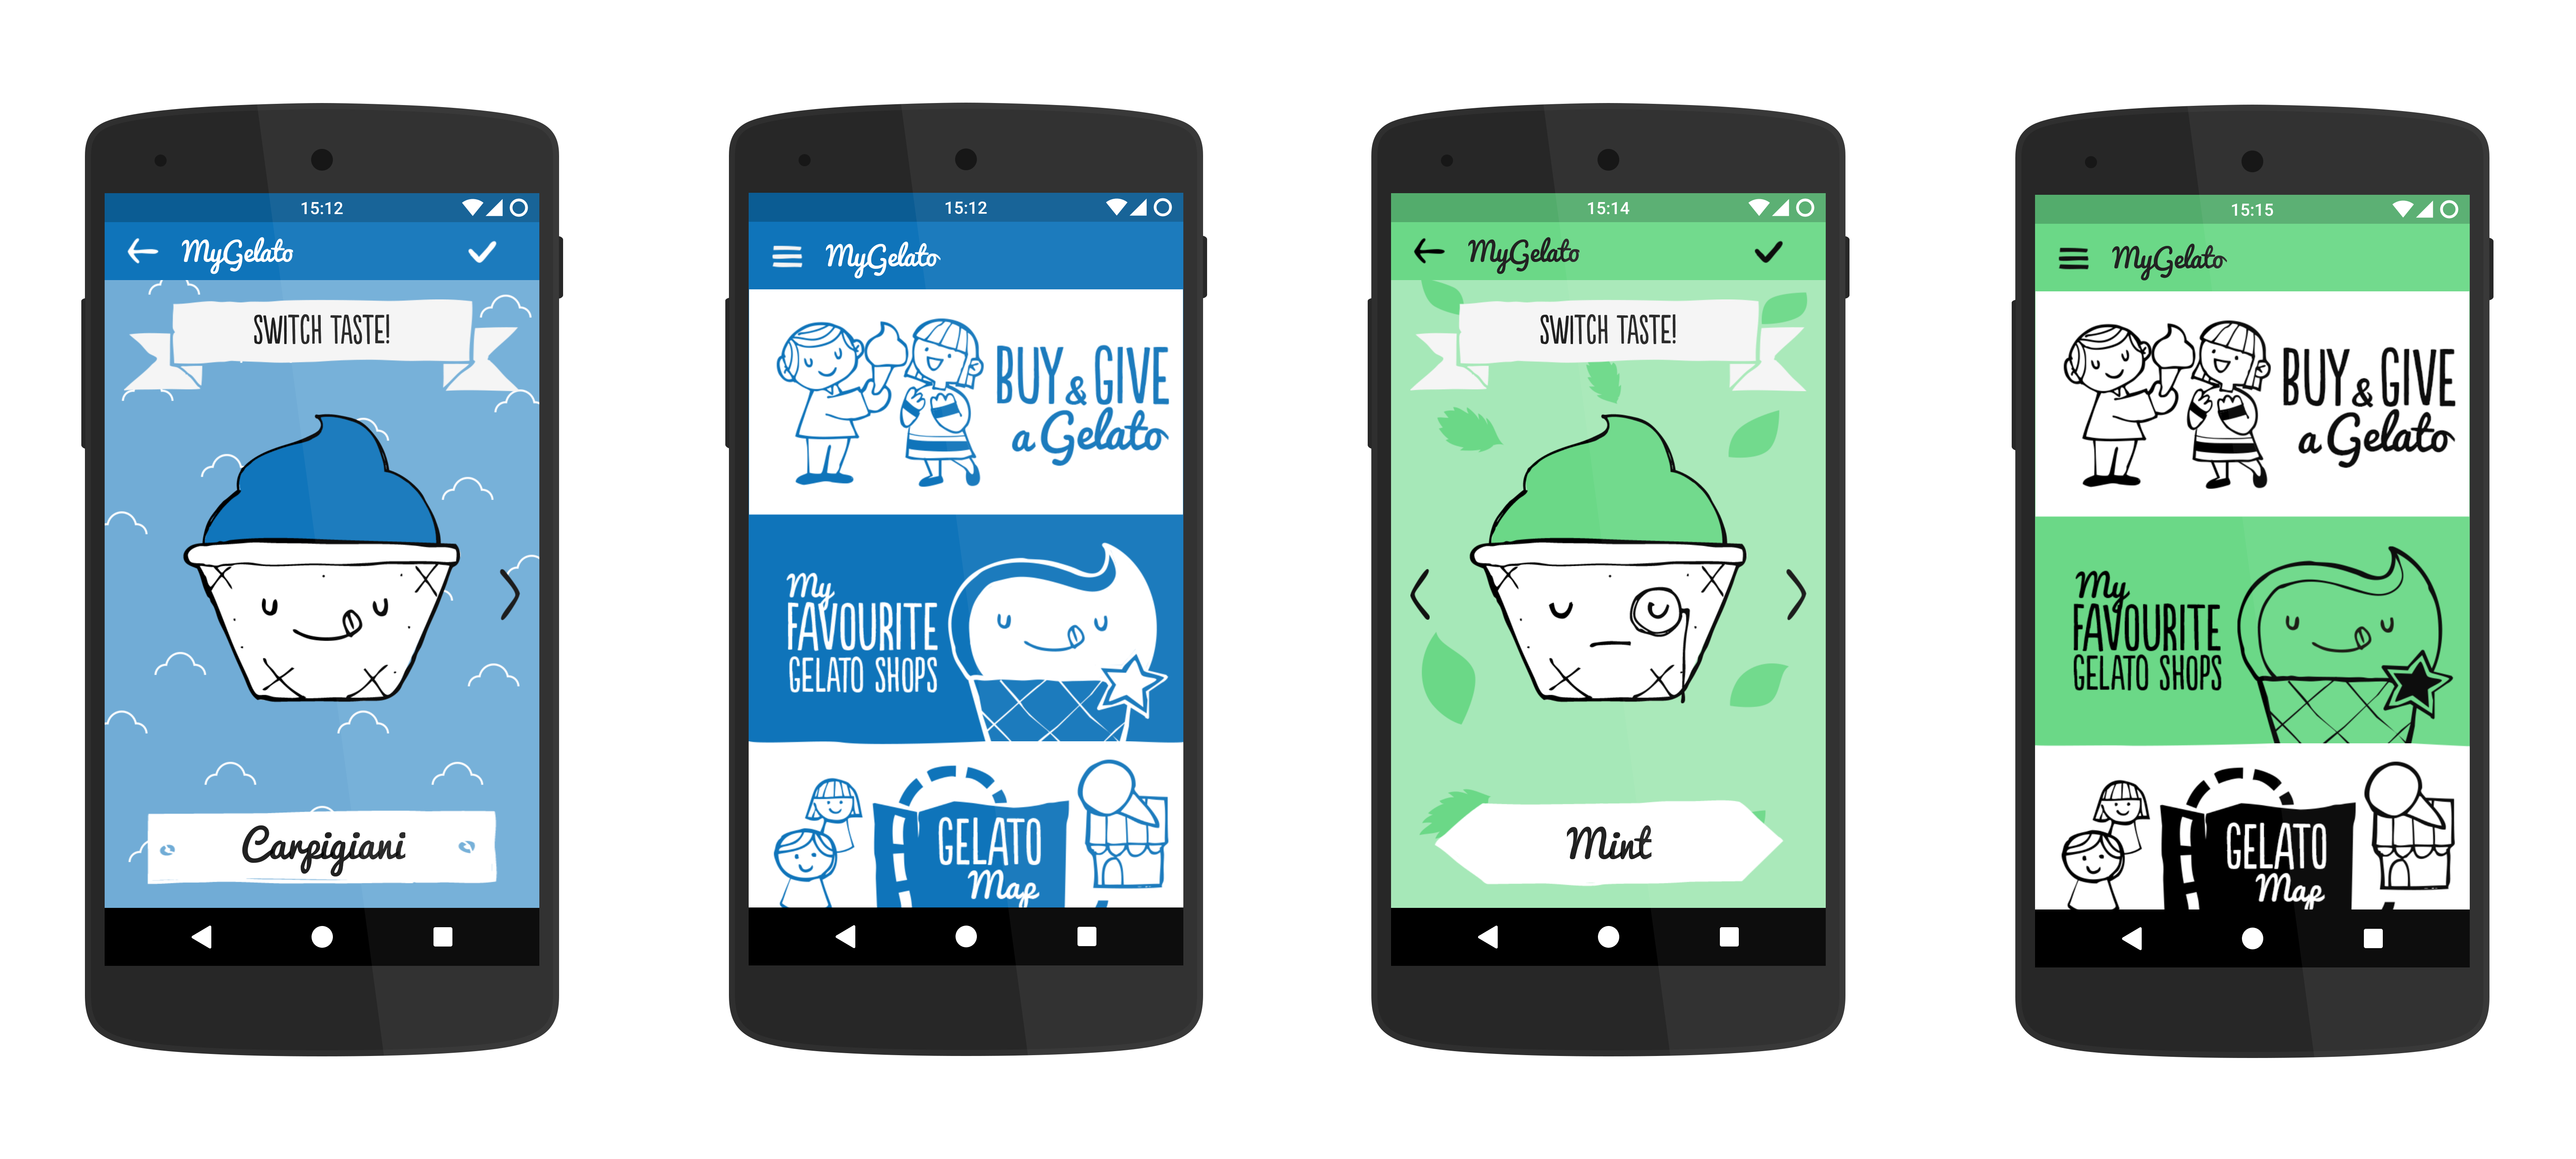
\includegraphics[scale=0.06]{/home/tommaso/Documents/Tesi/thesis/images/temi}\caption{\label{fig:Temi}Temi}
\end{figure}


\section{Network}

Tutte le funzionalità di collegamento al backend tramite API Rest
sono state raccolte e incapsulate all'interno di un unico componente
\emph{Network} utilizzato ad ogni chiamata server in maniera standardizzata.
Sfruttando la libreria OkHttp si è potuto semplificare la gestione
delle chiamate con protocollo Http potendo incapsulare il risultato
in un classe \emph{Result} contenente i dati sia in caso di successo
sia in caso di errore.

Le API Rest rese disponibili dal backend hanno permesso di standardizzare
le chiamate richiedendo ad ogni chiamata l'inserimento solo del metodo,
dei parametri da inviare e dell'eventuale payload. Anche la gestione
degli errori grazie ai codici identificativi Http hanno reso la gestione
di tutti gli errori semplificata così da poter visualizzare un messaggio
di errore il più specifico possibile e localizzato in base alla lingua
utilizzata sul device.

L'utilizzo di una libreria esterna molto performante ha permesso di
evitare l'utilizzo delle libreria Apache che, anche se elemento fondamentale
della programmazione Java in generale, nello specifico dello sviluppo
Android sono molto limitanti riguardo alla compatibilità con tutte
le versioni commercializzate e rende il codice piuttosto legato al
backend con cui ci si collega.

Per la gestione della risposta di una richiesta al server la possibilità
di utilizzare il \emph{Diamond Operator} ha permesso di utilizzare
lo stesso oggetto di tipo Result anche con risultato di tipo differente,
come per esempio i dati relativi ad un utente o ad una carta promozionale.
In questo modo tutte le chiamate server che venivano effettuate all'interno
delle sezioni dell'applicazione potevano essere replicate ed adeguate
facilmente al contesto senza dover riscrivere ogni volta il codice
necessario al funzionamento di una particolare sezione.

\inputencoding{latin9}\begin{lstlisting}
public class Result<T, E> {
    public T result = null;
    public E error = null;
    public Result(T result, E error) {
        this.result = result;
        this.error = error;
    }
}
\end{lstlisting}
\inputencoding{utf8}
L'utilizzo di un middleware così sviluppato per ogni chiamata al backend
ha permesso anche di inserire alcuni controlli su ogni richiesta inviata
dall'applicativo, per esempio la possibilità di verificare che le
chiamate autenticate non dessero come risultato il codice 401 in caso
di utente non autorizzato; situazione che invoca il logout dell'attuale
utente dall'applicazione.

L'utilizzo dell'oggetto Network, che espone i metodi statici necessari
all'utilizzo delle sue funzionalità in ogni punto dell'applicazione,
è stato ogni volta inserito all'interno di un componente \emph{AsyncTask}
che permette l'esecuzione di un blocco di codice in maniera asincrona
dal processo principale, migliorando di gran lunga le performance
dell'applicativo.

\section{Utente}

Lo sviluppo della sezione legata all'utente è iniziata con la realizzazione
di un modello, definito all'interno della classe \emph{User}, che
racchiude tutte le informazioni legate ad un account (mostrate nel
codice CODICE per come sono implementate all'interno del modello).
Utilizzando Realm è stato possibile definire un oggetto che lo rappresenta,
mantiene in locale sul dispositivo tutti i dati inseriti e mette a
disposizione un insieme di funzioni utili per la gestione del database.

\inputencoding{latin9}\begin{lstlisting}
@PrimaryKey
public String uuid;

public String firstName;
public String lastName;
public String email;
public String avatar;
public String uid;
public String client;
public String token;
public String provider;
public boolean shop;
\end{lstlisting}
\inputencoding{utf8}
La sezione per la gestione del proprio account e delle funzioni di
autenticazione sono inserite in una parte del menù laterale (\emph{NavigationDrawer})
della pagina principale dell'applicazione, permettendo di verificare
se si è effettuato o meno l'accesso rapidamente. Si è inserito un
header in cui sono visibili un'immagine circolare, un messaggio di
benvenuto e un bottone per eseguire l'accesso e una volta che l'utente
sarà autenticato saranno invece visibili l'avatar, il nome, un'icona
per accedere alla schermata di modifica dell'account e il bottone
per eseguire il logout.

Si è poi implementata un'unica schermata dalla quale si può accedere
al login tramite credenziali personali (\emph{EmailLogin}), al login
tramite social network (\emph{FacebookLogin}), alla registrazione
di un nuovo account (\emph{SignUp}) e si verrà reindirizzati a questa
sezione ogni volta che l'utente tenterà di eseguire delle azioni in
cui è necessario aver eseguito l'accesso senza essere autenticato.

Ogni azione che si vuole compiere, come per esempio l'accesso tramite
credenziali, deve è gestito all'interno dell'applicazione in modo
molto accurato: ogni campo di input è stato controllato in modo da
attuare una validazione anche lato client informando in maniera diretta
l'utente nel caso in cui i dati inseriti non siano corretti. A seguito
dell'invio di ogni form viene eseguita una chiamata alle API del backend
tramite l'interfaccia di supporto \emph{Network} implementata in modo
che ritorni eventuali messaggi di errore in maniera standardizzata.

Tutte le schermate facenti parte della sezione del Login sono state
create con un tema differente da quelli disponibili volendo creare
una separazione anche visiva tra i sistemi di marketing ed e-commerce
e le funzionalità legate all'utente che sono concettualmente parallele
ai flussi logici dell'applicazione e a un livello maggiore di generalità.

Nel momento in cui l'utente esegue il login vengono aggiornate sul
device le informazioni legate all'account, creando un oggetto Realm
partendo dal modello, incapsulando ogni informazione scaricata dal
server così che ogni sezione dell'applicativo possa accedervi localmente.
L'autenticazione e il logout sono funzioni gestite in maniera centralizzata
grazie ad un \emph{helper} che incapsula tutte le operazioni per far
si che nessun dato sensibile rimanga salvato in locale a seguite della
disconessione dell'account e non vi siano casi di incosistenza tra
le informazioni presenti in locale e sul server.

L'accesso permette inoltre di accedere ad alcune sezioni dell'applicazione
che altrimenti non si potrebbero utilizzare poichè ogni chiamata alle
API deve essere corredata delle informazioni legate all'utente che
esegue una determinata azione. Per questo motivo nel menù laterale
della navigazione principale dell'applicazione alcuni elementi sono
disabilitati finchè l'utente non esegue l'autenticazione, come mostrato
anche in figura FIGURA insieme agli elementi presentati in questo
capitolo.

\section{Shop}

Ogni gelateria inserita all'interno del circutio MyGelato è formalizzata
concettualmente come un oggetto \emph{Shop}, sia all'interno del frontend
sia sul backend, che incapsula tutte le informazioni disponibili al
download di volta in volta, anche qui presentati sotto forma di codice
per rendere più completa la descrizione delle variabili utilizzate.

\inputencoding{latin9}\begin{lstlisting}
@PrimaryKey
public String uuid;

public double latitude;
public double longitude;
public String name;
public String address;
public String phone;
public String status;
public boolean canBurnCoupons = false;
public boolean myGelatoShop = false;
\end{lstlisting}
\inputencoding{utf8}
Le informazioni riguardanti le gelaterie sono essenziali per la fruizione
dei contenuti all'interno del sistema di marketing digitale e per
la selezione dell'esercizio all'interno di quello di e-commerce. La
gestione e il salvataggio in locale degli Shop all'interno dell'applicazione
è stato necessario poichè in molti casi dati devono poter essere accessibili
anche offline per quanto riguarda le operazioni che non richiedono
un collegamento istantaneo con il backend, come per esempio la visualizzazione
degle esercizi preferiti.

È stato quindi creato un modello per l'oggetto Shop sempre derivante
da un oggetto Realm così da sfruttare tutta la potenza della libreria
per il salvataggio e la gestione dei dati in database. Il download
delle informazioni sul device avviene all'interno della schermata
della Ricerca e avviene in background poichè avviata in maniera asincrona,
a causa della grossa mole di dati da dover scaricare. Ad ogni ricerca
infatti le gelaterie vengono nuovamente scaricate così da avere sempre
tutte le informazioni aggiornate, creando però un collo di bottiglia
in termini di prestazioni che verrà spiegato e gestito nel dettaglio
nel capitolo successivo.

\section{Ricerca}

\section{Marketing Digitale}

Il primo flusso logico principale ad essere stato implementato è stato
quello del marketing digitale poichè legato solo in parte alla presenza
di un utente registrato e autenticato all'applicazione; sono quindi
presenti alcune operazioni comunque disponibili anche senza aver eseguito
il login.

La prima sezione ad essere implementata è stata quella legata alla
visualizzazioni delle carte del Mastro Gelatiere poichè il numero
delle promozioni disponibili era da visualizzare anche all'interno
della navigazione principale e quindi la richiesta per scaricarle
doveva essere presente anche all'interno della schermata iniziale
dell'applicazione.

Per ottenere un maggiore riutilizzo del codice si è scelto di creare
una stessa sezione per visualizzare sia le carte del mastro gelatiere
sia quelle delle singole gelaterie ottenendo una visualizzazione differente
in base al collegamento (\emph{Intent}) che avrebbe portato l'utente
all'interno della sezione. Allo stesso modo si è utilizzato uno stesso
modello per entrambe le carte definendo un elemento Realm di nome
\emph{Card} che incapsula i dati necessari all'utilizzo delle carte
nel sistema differenziandole grazie ad un flag presente anche nel
modello fornito dal backend.

Avendo quindi implementato la visualizzazione delle carte scaricate
tramite chiamata alle API, nella schermata appena descritta, è stato
semplice eseguire il passaggio successivo che dalla visualizzazione
della singola gelateria portava alle proprie carte promozionali: all'interno
della finestra informativa con i dati dello shop all'interno della
ricerca si sono inserite un'icona che funge da collegamento alle carte
un'icona per aggiungere ai preferiti il singolo esercizio.

Per il salvataggio offline dei preferiti si è però dovuto creare un
secondo modello all'interno del database \emph{Favorite} che semplicemente
identifica gli esercizi salvati tra i preferiti in modo che queste
informazioni rimangano salvate in locale sul dispositivo anche senza
che un utente che si sia loggato. L'inserimento di un flag all'interno
del modello degli shop non avrebbe funzionato poichè sarebbe stato
sovrascritto ad ogni aggiornamento degli shop durante il download
e la modifica con le informazioni sul server.

Una volta che una gelateria viene aggiunta ai preferiti, nel caso
l'utente si sia autenticato verrà eseguita una chiamata al server
che attiverà la ricezione di notifiche push e in automatico verrà
anche aggiunto un controllo per il geofencing sul dispositivo, entrambe
le funzioni sono spiegate nel dettaglio nel capitolo 4.6.2.

\subsection{Carte Promozionali}

L'implementazione delle carte promozionali ha seguito uno sviluppo
volto ad utilizzare lo stesso codice e le stesse visualizzazioni sia
per la la presentazione delle carte legate al singolo esercizio sia
per quelle del mastro gelataio. Prima di tutto si è quindi realizzato
il modello in Realm chiamato \emph{Card} contenente le principali
informazioni legate alla carta: 

\inputencoding{latin9}\begin{lstlisting}
@PrimaryKey
public String uuid;

public String name;
public String title;
public String imageUrl; 
public String shopUUID; 
public String cardDescription; 
public String link;
public String phone; 
public Long start; 
public Long end;
...
\end{lstlisting}
\inputencoding{utf8}
È stata creata una schermata unica per la visualizzazione delle carte
affiancate, grazie all'utilizzo di un \emph{ViewPager}, con un layout
di ogni pagina elaborato dove ogni carta mostra la propria immagine
e al click su un'icona in basso a destra ruota su se stessa per permettere
di leggere la descrizione ed eventualmente ottenere nuove informazioni
tramite il link proposto. Nel caso vi sia la presenza di un video
il tap sull'immagine porterà alla visualizzazione online della risorsa
resa disponibile tramite url.

Il download delle informazioni deve avvenire all'apertura della schermata
grazie ad una richiesta alle API in background così da non bloccare
il dispositivo dell'utente. Tutti i dati scaricati vengono salvati
in locale così da essere disponibili anche offline e nel caso di modifiche
saranno aggiornati eliminando le promozioni non più disponbili perchè
scadute.

Nel caso delle carte del mastro gelatiere il procedimento di richiesta
dei dati deve essere eseguito, come già detto, anche all'interno della
schermata principale poichè il numero delle carte è da visualizzare
all'interno dell'immagine del menù che rimanda alla sezione del mastro
gelatiere. Inoltre nel caso di un utente con autenticazione effettuata
verrà registrato il dispositivo sul server per la ricezione di una
notifica push ogni volta che sarano pubblicate nuove promozioni, funzionalità
spiegata nel dettaglio nel capitolo successivo.

\subsection{Preferiti}

Il primo sviluppo legato alla sezione dei preferiti è stata quella
della gestione dell'aggiunta e della rimozione di una gelateria come
esercizio d'interesse tramite un'icona all'interno della visualizzazione
della ricerca con cui l'utente può salvare localmente le sue preferenze.
Successivamente si è implementata la sezione dell'applicazione che
permette la visualizzazione e la gestione della lista degli esercizi
preferiti, direttamente raggiungibile dalla navigazione principale.

L'utente può aggiungere una gelateria ai preferiti cliccando sull'icona
della stella presente nella finestra di informazioni visualizzata
all'interno della ricerca degli shop una volta selezionatone uno.
L'aggiunta, come anche la rimozione, aggiorna immediatamente sia la
mappa modificando il marker mostrato a video e anche la lista dei
preferiti.

Grazie all'utilizzo del modello \emph{Favorite} è possibile accedere
ai codici identificativi degli Shop preferiti così da richiamarli
dal database in locale visualizzando tutte le principali informazioni
legate al sistema di marketing e dando la possibilità di accedere
alle carte promozionali o direttamente al \emph{dialer }selezionando
il recapito telefonico, se presente.

Avendo gestito l'aggiunta e la rimozione dei preferiti grazie ad un
sistema centralizzato che racchiudeva tutte le operazioni necessarie
è stato abbastanza intuitivo poter inserire un middleware che gestisse
l'aggiunta e la rimozione delle funzionalità riguardanti l'iscrizione
alle \emph{Notifiche Push} ricevute del server e del \emph{Geofencing}
gestito dal dispositivo.

Per l'implementazione della funzinalità di notifiche push si è scelto
di utilizzare i servizi resi disponibili da Google stessa utilizzando
inizialmente \emph{Google Cloud Messaging} per poi passare ad utilizzare
il servizio \emph{Firebase}, nuovo applicativo appena reso disponbile
e sicuramente più innovativo e aggiornato. Per far dialogare in maniera
bidirezionale l'applicativo e il server nel momento in cui un utente
esegue il login all'applicazione viene attivato Firebase richiedendo
al server un token che verrà poi passato al sistema di gestione delle
notifiche, incluso al'interno del codice come libreria, che si metterà
in ascolto di eventuali messaggi. Viene presentato per semplificazione
solo l'inizializzazione parziale del sistema di ascolto di notifiche
push e si rimanda alla documentazione completa per ottenere le informazioni
necessarie alla descrizione dell'implementazione.

\inputencoding{latin9}\begin{lstlisting}
FirebaseApp.initializeApp(
    this,
    FirebaseOptions.fromResource(this)
);
\end{lstlisting}
\inputencoding{utf8}
Ogni volta che l'utente aggiungerà e rimuoverà un preferito verrà
quindi eseguita una chiamata al backend con lo scopo di informarlo
della modifca attivando o disattivando rispettivamente la ricezione
delle notifiche push. In questo modo nel momento in cui sarà disponibile
una nuova carta promozionale per quello \emph{Shop} verrà visualizzata
una notifica sul device che permetterà all'utente di accedere direttamente
alla sezione delle carte promozionali specifiche per quell'esercizio.

Allo stesso tempo, solo a livello applicativo in locale sul device
verrà inoltre sottoscritto al sistema una richiesta di geofencing
che produrrà un \emph{Intent} ogni qual volta l'utente rimarrà entro
l'area di 5 kilometri da una gelateria presente tra i preferiti, il
quale verrà gestito per mostrare anche in questo caso una notifica
che permetterà di accedere invece alle informazioni della gelateria
all'interno della lista dei preferiti. Ovviamente per i dispositivi
con le ultime versioni di Android sarà necessario richiedere anche
in questo caso la possibilità di accedere alla localizzazione come
fatto all'interno della ricerca.

Nello snippet di codice si può vedere come l'applicazione si registra
al servizio di Geofencing del sistema una volta che una gelateria
\emph{shop} viene inserito tra i preferiti, situazione che va oltretutto
ripetuta ogni volta che il device dell'utente viene riavviato.

\inputencoding{latin9}\begin{lstlisting}
mGeofenceList.add(new
    Geofence.Builder()  
      .setCircularRegion(                                             
         shop.latitude,                                             
         shop.longitude,                                             
         GEOFENCE_RADIUS_IN_METERS                                     
      )                                     
      .setLoiteringDelay(2 * 60 * 1000)                                     
      .setTransitionTypes(Geofence.GEOFENCE_TRANSITION_DWELL)                                     
      .build()
);
\end{lstlisting}
\inputencoding{utf8}

\section{E-Commerce}

Il sistema di e-commerce è stato l'ultimo tassello dell'applicazione
che ha concluso il lavoro di sviluppo di questo elaborato. Si è trattato
di unificare parte delle componenti già implementate creando un workflow
che permetta all'utente di comprare e utilizzare i coupon digitali
in sicurezza e con facilità.

La prima fase è stata legata alla rappresentazione formale dei buoni
acquistati da un determinato account e di quelli invece disponibili
all'acquisto legati ad una determinata gelateria, in particolare è
stato importante valutare quali informazioni mantenere sempre in locale
per non inficiare la consistenza dei dati presenti sul dispositivo
rispetto a quelli online.

Definita la struttura degli elementi che si sarebbero andati ad utilizzare
si è creata la sezione dedicata alla gestione dei coupon personali
disponibili ad ogni utente, ovviamente legando ogni funzione all'avvenuta
autenticazione tramite account MyGelato. Questa sezione permette di
avere una visione completa delle proprie informazioni aggiornate costantemente
rispetto ai dati presenti sul server online.

Le funzioni legate al sistema di e-commerce comprendono l'utilizzo
di account e dispositivi diversi che interagiscono tra di loro e che
non devono assolutamente creare casi di incosistenza sul database
sia online sia offline in locale sui device utilizzati.

Per rendere accessibile all'utente l'accesso alle funzioni di acquisto
e di riscatto di un buono in maniera diretta si sono inseriti all'interno
della navigazione principale dell'applicazione i collegamenti a queste
sezioni insieme ad un bottone flottante che riporta alla gestione
dei coupon; nel caso si sia effettuato l'accesso con un account di
tipo gelatiere si verrà riportati invece alla sezione per la validazione
dei buoni.

\subsection{Coupon}

Per formalizzare il concetto di buono acquistato da ogni utente si
è scelto di creare il modello \emph{Coupon}, estensione di un oggetto
Realm, che incapsula tutte le informazioni disponibili visualizzate
sotto forma di codice all'interno dello snippet di codice successivo.
Sfruttando Realm inoltre le operazioni di salvataggio sul database
sono particolamente semplificate e grazie alla corretta gestione delle
transizioni viene assicurata un alto livello di sicurezza rispettando
le proprietà logiche \emph{ACID}.

Ogni coupon è unico grazie a un codice identificativo, possiede alcune
informazioni importanti come l'acquirente e l'attuale propietario,
la data di vendita e anche alcune informazioni non direttamente utili
all'utilizzo all'interno dell'applicativo frontend che però vengono
trasmesse per completezza e nel caso possano essere necessarie per
futuri sviluppi. 

Nel momento in cui si accede alla sezione per la gestione dei coupon
vengono scaricati tutti i dati in background così da aggiornare il
database locale e grazie ad una funzionalità di Realm, una volta eseguito
un update sulla base dei dati vengono ricaricate alcune view dell'interfaccia
andando a riempire con tutte le informazioni le tre liste presenti:
Coupon Validi, Coupon Ricevuti e Lista Completa dei Coupon.

Come si può vedere in figura \ref{fig:Coupon}, ogni coupon visualizza
alcune informazioni di base e sono presenti i collegamenti diretti
per l'utilizzo e lo share tramite altri canali di comunicazioni. Selezionando
la parte sinistra del buono si verrà reindirizzati all'interfaccia
di utilizzo presentata nel dettaglio al capitolo 4.7.4 mentre cliccando
sulla parte destra si verrà invitati a chiedere il metodo di condivisione
da utilizzare.

Nel caso in cui un coupon sia stato già utilizzato non sarà possibile
eseguire nessuna delle due operazioni e la parte destra dell'immagine
verrà nascosta per dare l'impressione di un buono strappato dopo averne
usufruito. Per ottenere coerenza da questo punto di vista ad ogni
passaggio di schermata vengono ricercate eventuali modifiche sul server
sempre per mantenere la coerenza dei dati interni al sistema MyGelato.

\begin{figure}

\caption{\label{fig:Coupon}Coupon}

\end{figure}


\subsection{Acquisto}

Il sistema di acquisto di un coupon è stato quello più complesso poichè
doveva operare con più di un componente esterno all'applicazione mantenendo
però ad ogni passaggio un alto livello di sicurezza senza inficiare
alla consistenza dei dati della piattaforma MyGelato: a esempio una
volta scelto lo shop, per modifcare la gelateria si perdono le scelte
successive riportando l'utente al passaggio iniziale per non rischiare
incosistenze nel sistema. Si è poi analizzato ogni singolo passaggio
per poter guidare l'utente durante ogni step mostrando a video di
volta in volta solo ciò che era richiesto.

La schermata di acquisto di un coupon è stata creata in modo che sia
raggiungibile direttamente dal menù di navigazione princiapale, ma
nel caso in cui l'utente non abbia eseguito l'autenticazione viene
rimandato alla schermata di login dove vengono richieste le credenziali
per poter continuare. In questo modo solo gli utenti registrati alla
piattaforma hanno la possibilità di effettuare un acquisto che richiede
un collegamento con il backend dove sono necessarie le credenziali
di autenticazione.

Come si può vedere in figura FIGURA dopo l'helper iniziale viene richiesto
all'utente di scegliere da quale gelateria vuole acquistare un coupon
e, come già specificato, si verrà reindirizzati alla mappa di ricerca
con un Intent d'avvio contenente alcune opzioni che disabiliteranno
la visibilità degli shop in cui non è abilitato il sistema di e-commerce
e sostituiranno alle icone presenti nella finestra di dettaglio un'icona
per la selezione dell'esercizio. Una volta che l'utente avrà effettuato
la selezione verrà riportato sulla schermata di acquisto dove saranno
mostrati i dettagli della gelateria e verrà invece visualizzata la
possibilità di scegliere il metodo di pagamento.

Per effettuare questa operazione l'applicazione esegue due chiamate
differenti al server, una nelle quali richiede il codice identificativo
dell'utente rispetto alla libreria di e-commerce Stripe, che servirà
per richiedere i metodi di pagamento disponibili dell'utente, e scarica
inoltre anche i coupon disponibili per l'esercizio scelto. In questa
caso i coupon sono salvati all'interno di un modello \emph{AvaiableCoupon
}poichè le informazioni necessarie sono ridotte rispetto al singolo
coupon dell'utente; i dati scaricati inoltre non vengono salvati sul
database del device poichè una volta usciti dalla schermata non sono
più utili ed è in ogni caso necessario ogni volta riscaricarli nel
caso siano stati modificati.

Lo step successivo con cui l'utente può procedere è la scelta del
metodo di pagamento che verrà effettuato in una schermata separata
dove sarà visualizzata la lista dei motodi precedentemente inseriti
dall'utente e scaricati tramite chiamata al backend. Gli unici dati
verranno ricevuti saranno però parziali e utili solo al riconoscimento
dei dati presenti: ultimi numeri della carta inserita e la data di
scadenza. Oltre alla possibilità di scegliere una delle opzioni già
presenti l'utente potrà aggiungere una nuova carta grazie ad una schermata
separata, differenziata anche nella grafica, dove i dati non verranno
memorizzati ma inviati direttamente alla libreria di Stripe che si
occuperà di validare i dati e aggiornare i dati presenti sul backend.
Si verrà infine reindirizzati alla schermata precedente dove le opzioni
saranno aggiornate.

Scelto il metodo di pagamento si verrà riportati sulla schermata di
acquisto dove saranno visualizzati i dati essenziali dell'opzione
scelta dando, come nel caso dello shop, la possibilità di modificare
la decisione presa. Infine l'ultima decisione sarà quella riguardante
il coupon da acquistare grazie alla visualizzazione di quelli disponibili.

Sotto il collegamento alla scelta del motodo di pagamento è quindi
presente un \emph{ViewPager} che visualizza i coupon disponibili specifici
per la gelateria scelta mostrando i dettagli principali: nome, descrizione,
prezzo e valuta. In questo caso la scelta verrà effettuata scorrendo
sullo slide in modo che al centro della schermata vi sia quello scelto
dall'utente.

Concluse tutte le scelte l'utente potrà procedere con l'acquisto che
si tratterà di una nuova chiamata alle API del server in modo che
grazie anche all'utilizzo del codice Stripe sia dell'utente che dello
shop potrà effettuare la transizione e aggiungere il coupon a quelli
legati all'account utilizzato. Nel caso di errori verrà visualizzato
un messaggio e si potrà ritentare l'operazione, altrimenti se non
vi dovessero essere problemi si verrà reindirizzati alla schermata
di gestione dei coupon personali.

\subsection{Condivisione e Riscatto}

Il meccanismo di condivisione e riscatto ha portato allo sviluppo
di funzioni complementari per un sistema e per l'altro che dovevano
sfruttare anche componenti a livello di sistema operativo. Per permettere
il dialogo tra due dispositivi differenti si è scelto di sfruttare
i canali di comunicazioni più comuni e diffusi anche tra gli utenti
medi in modo che il sistema di share sia il più facile possibile e
del tutto conforme al sistema di condivisione standard della piattaforma.
In genere questi metodi presuppongo una conoscenza da parte dei due
utenti che interagiscono, ma ci si è basati sul fatto che da specifiche
questo fosse una parametro valutato durante lo sviluppo del sistema
MyGelato.

Dalla lista di coupon disponibili l'utente ha quindi la possibilità
di cliccare sull'icona per la condivisone e verrà inviata una richiesta
- \emph{Intent} - a livello di sistema in broadcast per poter selezionare
il metodo che si preferisce per inviare il contenuto da scambiare:
un testo precompilato insieme ad un link che riporta ad una pagina
web esposta online dal backend. Il testo presenta brevemente l'oggetto
della condivisione e invita ad utilizzare il link per riscattare il
coupon specificato.

La pagina web a cui si viene reindirizzati riconosce il sistema operativo
dal quale ci si sta collegando per effettuare un redirect ad un link
particolare (\emph{mygelato://}) che verrà gestito in automatico dal
device con cui si sta visualizzando il sito. Nel caso in cui vi sia
installata sul device l'applicazione MyGelato allorà verrà avviata
la schermata di riscatto precompilata con i dati necessari, altrimenti
si verrà reindirizzati agli store principali per consigliare il download
dell'applicazione.

Il mezzo di identificazione del coupon condiviso è un codice alfanumerico
a sei cifre, il PNR, che viene condiviso in automatico insieme al
resto delle informazioni. Si è quindi creata la schermata per riscattare
un buono, sezione raggiungibile dirattamente dalla navigazione princiapale
dell'applicazione, dove è presente una view di input dove si deve
inserire il codice PNR; nel caso si arrivi sulla schermata tramite
il link descritto sopra allora il campo di input del codice sarà già
compilato.

Una volta inserito il codice, che verrà validato al momento con dei
controlli basilari, sarà effettuata una richiesta al server tramite
chiamata API che attuerà lo spostamento del buono da un utente all'altro.
Per entrambi gli account vi sarà quindi l'aggiormento delle informazioni
sul proprio dispositivo la prima volta che verranno richiesti i coupon
disponibili e l'utente che ha effettuato il riscatto verrà immediatamente
reindirizzato sulla schermata di lista dei coupon altrimenti, in caso
di fallimento dell'operazione, verrà notificato con un messaggio di
errore. 

La figura \ref{fig:Condivisione-e-Riscatto} mostra tutti i passaggi
principali per la condivisione e il riscatto di un buono seguendo
il flusso logico proposto all'utente ad ogni step, molti dei quali
anticipati da un'immagine informativa che esplica brevemente come
utilizzare ogni singola schermata.

\begin{figure}

\caption{\label{fig:Condivisione-e-Riscatto}Condivisione e Riscatto}

\end{figure}


\subsection{Utilizzo e Validazione}

L'ultimo passaggio del workflow di e-commerce è l'utilizzo pratico
dei coupon che si sono acquistati o che si sono riscattati perchè
condivisi da altri utenti. In questo processo entrato in gioco due
entità che sono utenti che spesso non entrano in contatto se non solo
per i pochi momenti che servono all'acquisto materiale del valore
del buono utilizzato. Questa situazione pone alcune limitazioni negli
strumenti utilizzati per la comunicazione tra i due dispositivi che
devono collaborare mantenendo uno stato costantemente consistente
sia sui device fisici che sul server.

Per superare questo ostacolo si è scelto uno strumento molto diffuso
che è l'utilizzo di un QR code che permette di generare un'immagine
a partire da un testo, in questo caso il PNR code lagato al coupon
che si vuole utilizzare, leggibile ed interpretabile da un qualsiasi
cellulare con un fotocamera. Chiunque abbia effettuato l'accesso all'applicazione
con account di tipo gelatiere potrà validare il coupon direttamente
tramite l'applicazione MyGelato grazie a una chiamata API al backend
che confermerà o meno l'avvenuta conclusione del processo senza problemi.

La sezione per generare e visualizzare il codice QR da mostrare in
gelateria è raggungibile cliccando sul singolo coupon all'interno
della gestione dei propri buoni. Questa schermata mostra una versione
del coupon a tutto schermo e, grazie ad una libreria esterna, inserisce
il codice QR all'interno del coupon in modo che sia ben visibile e
riconoscibile da qualsiasi software. Si deve quindi solamente mostrare
il dispositivo utilizzato a chi dovrà poi validare il buono. Non essendo
presente in questo caso una connessione bidirezionale con il backend,
per aggiornare la schermata una volta concluso il processo di utilizzo,
l'applicazione effettua un polling al server ogni cinque secondi per
verificare se il coupon sia stato utilizzato o meno.

Chiunque possieda un account di tipo gelatiere avrà nella navigazione
principale dell'applicativo il collegamento alla sezione per la convalida.
Verrà avviata immediatamente la fotocamera che, tramite una libreria
esterna, verificherà la presenza o meno di codici QR leggendoli. Dopo
una validazione semplice si effettettuerà la chiamata al server dando
poi la possibilità di convalidare altri coupon senza dover ritornare
ogni volta alla schermata iniziale. Nel caso in cui la fotocamera
sia già occupata da altri processi attivi sul dispositivo o nel caso
in cui l'utente abbia rimosso alcuni permessi all'applicativo verrà
visualizzato un messaggio di errore che comunicherà al proprietario
del device cosa fare per risolvere il problema.

A conclusione del processo di validazione di un coupon entrambi i
dispositivi verranno aggiornati per mantenere coerenza tra i dati
presenti sul sistema risolvendo così in maniera semplice il problema
principale del dialogo tra due dispositivi mentre verranno nel frattempo
applicati i passaggi commerciali totalmente all'interno del backend
avendo passato il codice identificativo del commerciante. 

La figura \ref{fig:Acquisto} permette di visualizzare i passaggi
fondamentali per l'utilizzo e la validazione di un buono, anche in
questo caso vengono visualizzati al primo avvio alcune immagini informative
per aiutare gli utenti nell'utilizzo delle funzionalità appena descritte.

\begin{figure}

\caption{\label{fig:Acquisto}Acquisto}

\end{figure}

\newpage{}
